\chapter{Product Description}
In this chapter we describe the product of our bachelor thesis and the main component of our application - the demonstrator web-application (front-end). We will focus mainly on the non-technical concepts as the next chapter will explain the technical implementation of the product.

\section{Application Overview}
In an essence, all the functionality of our application revolves around visualizing an election event of the CHVote protocol and guiding the users through the several phases of such an election event. A typical CHVote election event can be broken down into phases shown in figure \ref{Phases of an election-event}

\begin{figure}
\begin{center}
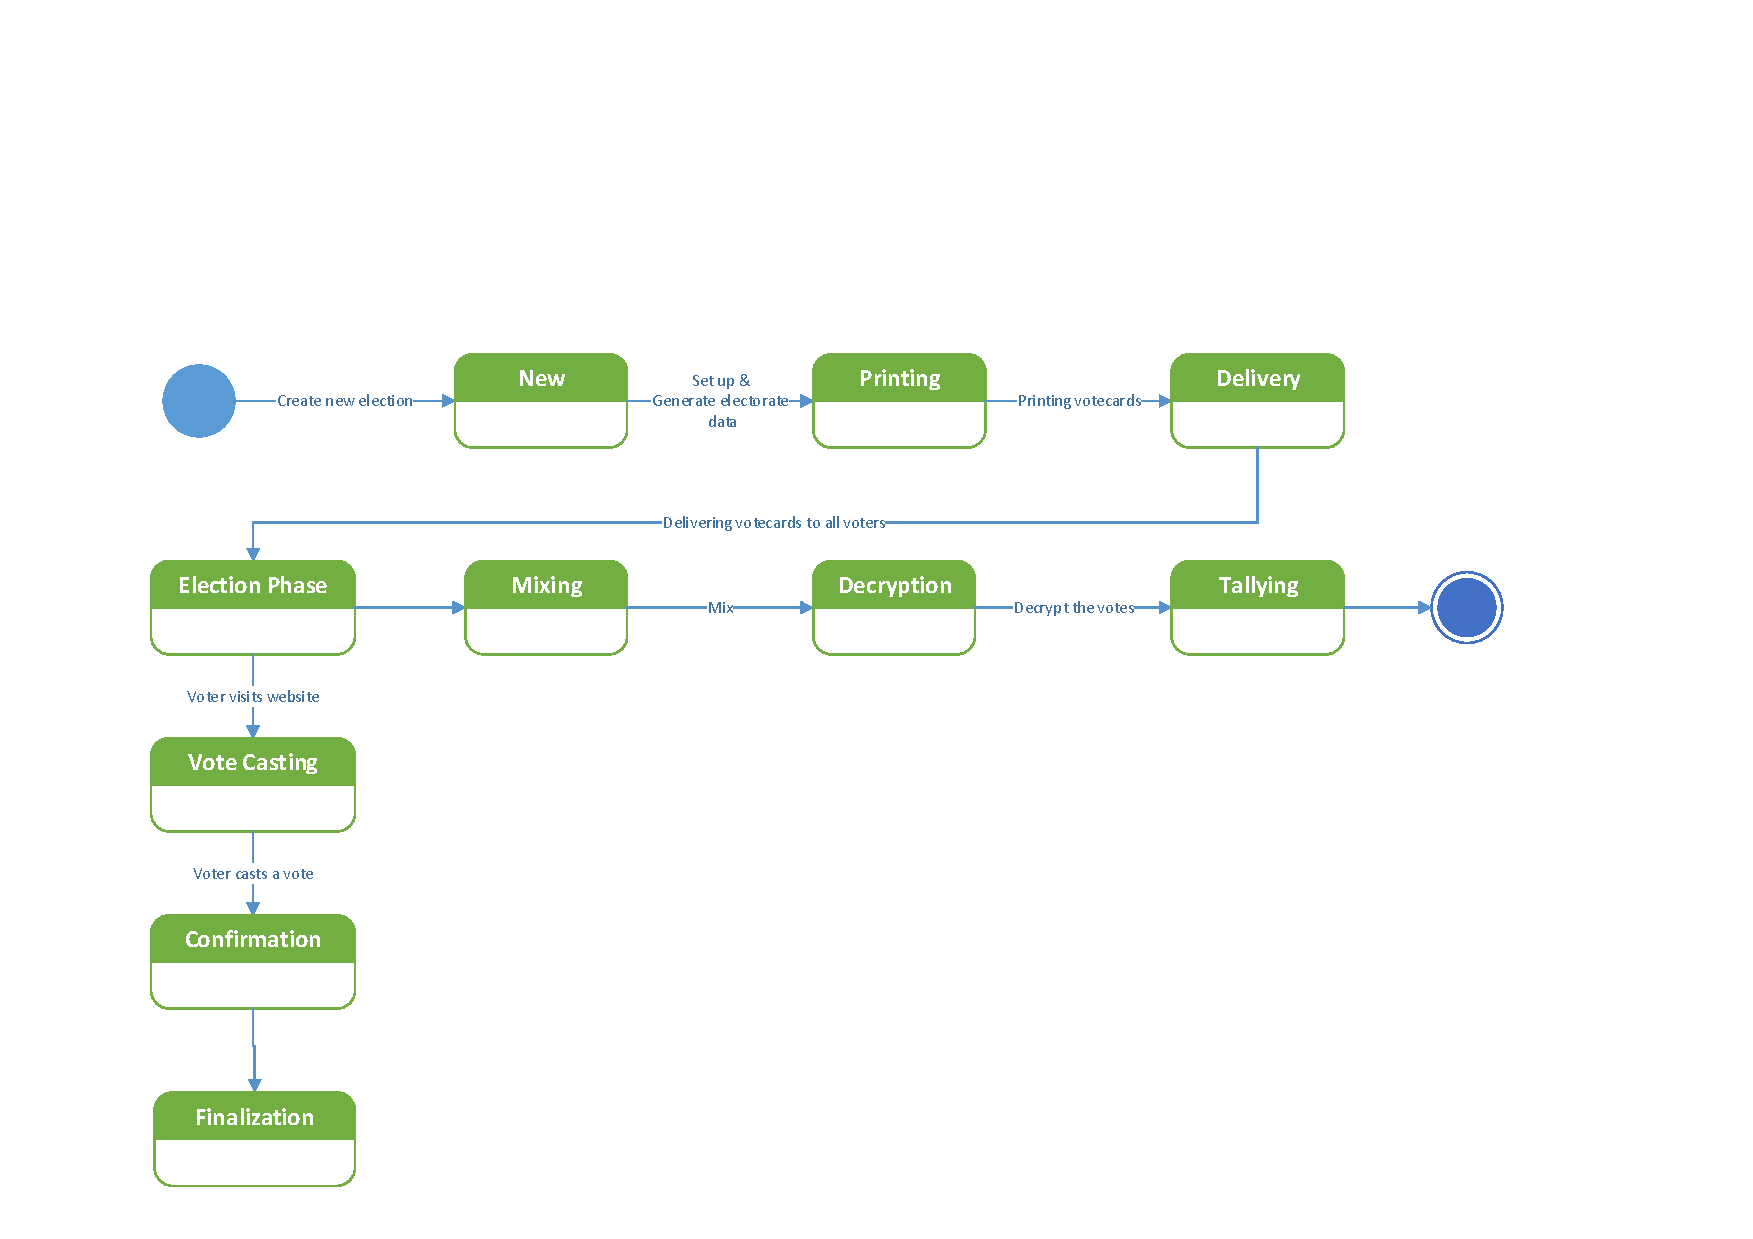
\includegraphics[scale=0.65]{assets/electionStatediagram.pdf}
\captionof{figure}{In our application, an election event consists of 7 different phases (green). During the election phase, a voter can be in 3 different phases (blue)}\label{Phases of an election-event}%
\end{center}
\end{figure}

To allow the users of our application to experience and get insights about the workings of the protocol, we wanted let them take the perspective of every actor of the protocol at any given time and during every phase of the election event. This is why we have divided our application into separate \textbf{views}, one for every actor:

Every actor involved in a CHVote election event has it's own set of data to be displayed and specific tasks and use-cases it has to perform. Most use-cases are only available during a particular phase.

\begin{itemize}
	\item \textbf{Election Overview}: The election overview shows in what phase the chosen election event is currently in. Additionally, a graphical schema shows how all the actors of the e-voting ecosystem are connected and who is currently in charge of performing an action.
\begin{figure}
\begin{center}
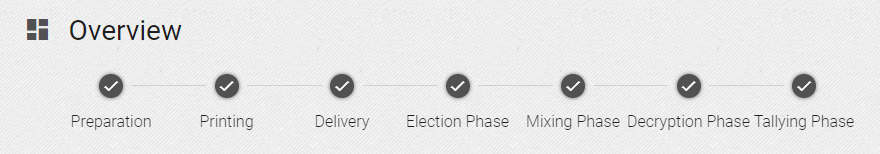
\includegraphics[scale=0.50]{assets/screenshots/overview.PNG}
\captionof{figure}{The election overview guides the user through the several phases of an election event and indicates what phases have been finished and what the next steps are.}\label{Election Overview}%
\end{center}
\end{figure}

	\item \textbf{Election Administrator View}: The view of the election administrator allows a user to set-up an election event, by configuring the number of voters, the elections including the candidates and the number of selections per election. Instead of providing these information every time an election event is set up, previously defined election presets can be applied or the parameters can be generated randomly.

The election administrator view is also the place where the elections can be tallied and the final result is determined during the post-election phase.
	\item \textbf{Printing Authority View}: In the printing authority view, the voting cards can be printed and displayed for every voter. Additionally, the voting cards can be sent to the voters.

	\item \textbf{Election Authority View}: The election authority view first lets a user choose one of the three election authorities he wants to observe. On the top, new tasks will pop up whenever an election authority needs to perform a specific task such as ballot- or confirmation checking or mixing and decryption.

Additionally, the view shows the data that an election authority knows. This concept of diving a view into tasks and data, can best been seen in figure \ref{Election Authority View} and has been used throughout the application and in almost every view.

\begin{figure}[p]
\begin{center}
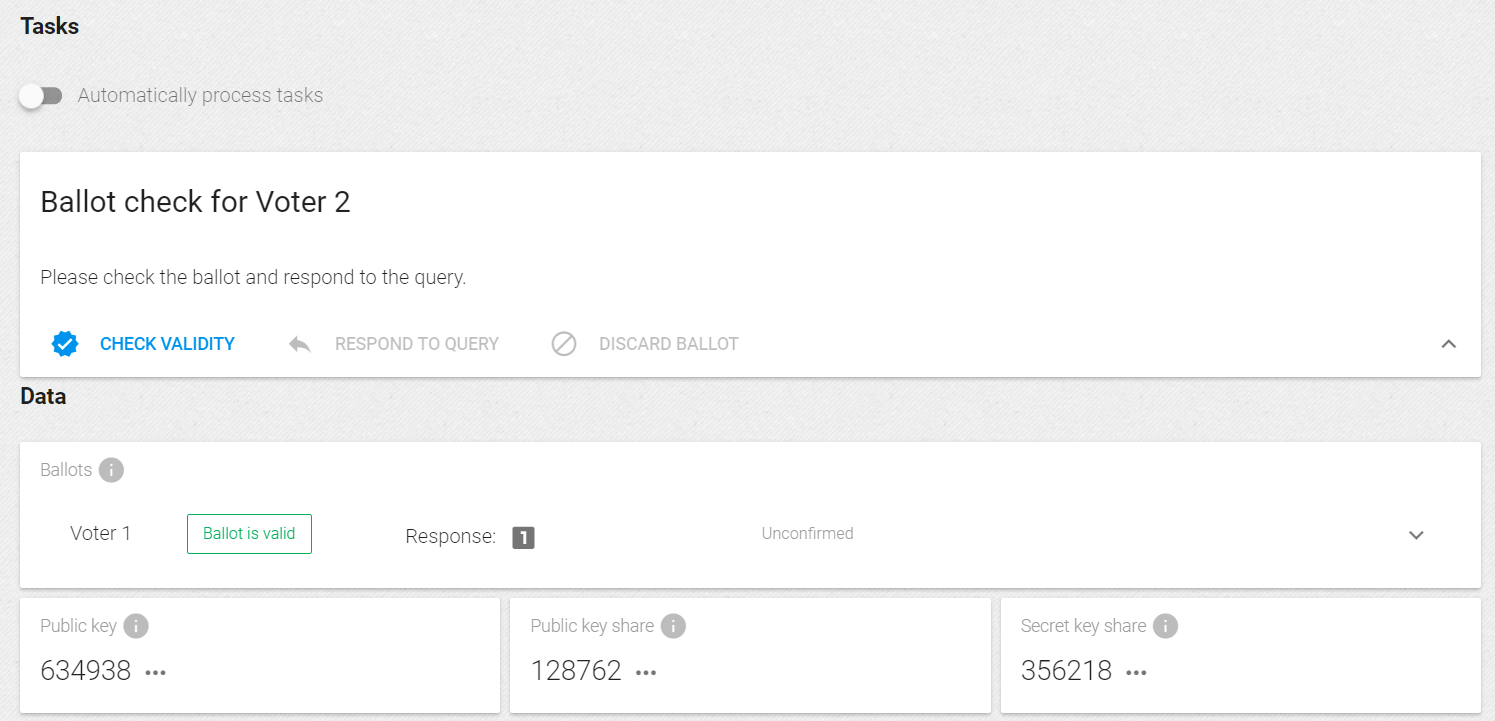
\includegraphics[scale=0.43]{assets/screenshots/view.png}
\captionof{figure}{The election authority view as an example of how we generally structure our pages: Most views are divided into a tasks part, which allows to perform the tasks of an actor, and a data part which shows what information about an election event the participant is in possession of. }\label{Election Authority View}%
\end{center}
\end{figure}

	\item \textbf{Voter View}
	In the voter view, the vote casting process can be done for every voter that has been previously generated. The view displays a candidate selection and code input form in the left, and a voters voting card in the right side. The voting cards codes are hidden behind a scratchcard if they are sensitive and private to the voter and can be applied to the form by clicking on them after they have been scratched open.

The voter view additionally has to consider the current phase of a voter e.g. if he has already casted a vote, if he already confirmed his vote or if he aborted the vote casting process.

	\item \textbf{Bulletin Board View} The bulletin board view always shows all the data that has been appended to the bulletin board by the other actors, such as the pre-election data, the ballots that the voters have casted, as well as all the proofs generated during the post-election phase.

	\item \textbf{Verifier View}: The view of the verifier becomes visible after the election result has been published to the bulletin board and the election event has reached its final stage. By clicking on the verify button, several checks can be executed and the result is display on the page.
\end{itemize}

All the views are accessible from a tab view displayed on the top of the page which serves as our standard mean for navigation, see figure \ref{Navigation}.

\begin{figure}[p]
\begin{center}
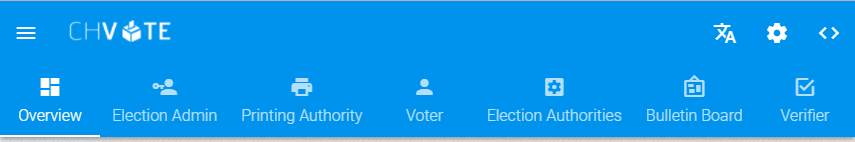
\includegraphics[scale=0.44]{assets/screenshots/navigation.png}
\captionof{figure}{The tab beyond the page header is the main control for navigating through the different pages. It also indicates where some interaction is required next by displaying an exclamation-mark icon in the respective actors tab}\label{Navigation}%
\end{center}
\end{figure}

From the use-cases, we tried to figure out all commonalities between the views: The views typically display the information known by the respective actor. Especially the bulletin board and election authorities will contain lots of information to be displayed. Most of the views have distinct tasks to be executed by the respective actor, such as casting a ballot in the voters view or confirming ballots from an election authorities view.

The content that a view displays, or in other words, the functionality an actor has access to, depend on the phase the election event is currently in: During the pre-election phase, the vote administrator needs to able to set up the election while in the tallying phase, he must be able to tally and determine the final result.


The following matrix shows all the possible combinations of views and phases.
%\begin{landscape}
%\begin{center}
%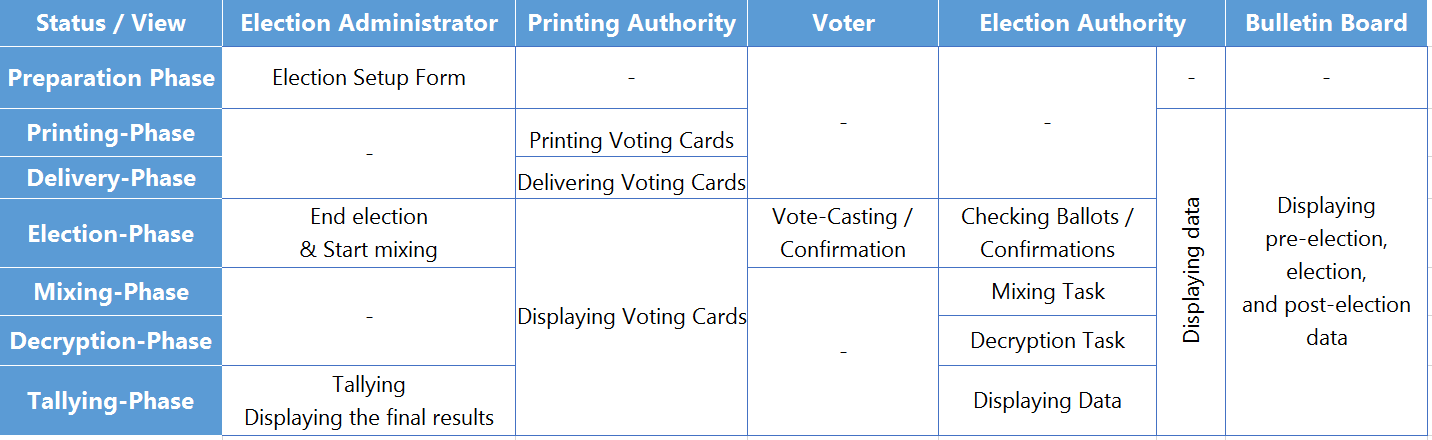
\includegraphics[scale=0.90]{assets/stateactormatrix.pdf}
%\end{center}
%\end{landscape}

\section{Design}
Given the rather large amount of complex data to be displayed, the main challenge of the project has been a well designed user interface that allows to display all important information while maintaining a clear overview.

To achieve this goal we tried to keep our design very minimalistic and follow the Google material design guidelines as much as possible by choosing an appropriate UI component framework. Even though mobile compatibility hasn't been a requirement, still it was nevertheless our goal to make the layout as responsive as possible such that it can at least be used from a mobile phone. The web-application is definitely optimized for desktop use.

Throughout our application we tried to establish common concepts regarding the look and feel and on how to display our data. One popular layout-concept of the google material guidelines is the card layout. Cards can be easily integrated in a responsive grid system, look modern and allow to visually group data. In addition, we used pushover menus, tooltips and pop-ups as they made it possible to hide lesser relevant information by default and display it only on demand of the user.

Before we started implementing our application, we have created mock-ups for most of the views, to discuss our ideas with our supervisors and incorporated their feed as well. The following screenshots are an extract of the mock-ups in which we tried to visualize how we imagined the resulting application to look like during the conceptual phase.

% Todo: Beispiel-Bild der Mockups %

Our conceptual work also involved the development of a small prototype / proof of concept, in which we have implemented one use case in a reduced extent with the envisaged frameworks and technologies to evaluate the technical feasibility. For more information about the languages and frameworks we have decided on, we refer to the next chapter.
